\documentclass[11pt]{article}
\usepackage{epsfig,psfrag}
\usepackage{amsmath}

\setlength{\textwidth}{6.2in}
\setlength{\oddsidemargin}{0.3in}
\setlength{\evensidemargin}{0in}
\setlength{\textheight}{8.7in}
\setlength{\voffset}{-.7in}
\setlength{\headsep}{26pt}
\setlength{\parindent}{10pt}
\begin{document}

\input{../latex/macros.tex}  % input some useful macros
\input{exermacros.tex}       % more macros for exercise formatting

% For exercises,
% set enumerate to give parts a, b, c, ...  rather than numbers 1, 2, 3...
\renewcommand{\theenumi}{\alph{enumi}}
\renewcommand{\labelenumi}{(\theenumi)}


% header:
\chapexercises{4}


\exercise[(Convergence of SOR)]{4.1}

The m-file \verb+iter_bvp_Asplit.m+ implements the Jacobi, Gauss-Seidel, and
SOR matrix splitting methods on the linear system arising from the boundary
value problem $u''(x) = f(x)$ in one space dimension.  

\begin{enumerate}
\item Run this program for each method and produce a plot similar to 
Figure~4.2.

\item The convergence behavior of SOR is very sensitive to the choice of
$\omega$ ({\tt omega} in the code).  Try changing from the optimal $\omega$
to $\omega = 1.8$ or 1.95.

\item Let $g(\omega) = \rho(G(\omega))$ be the spectral radius of the
iteration matrix $G$ for a given value of $\omega$.  Write a program to
produce a plot of $g(\omega)$ for $0\leq \omega \leq 2$.

\item From equations (4.22) one might be tempted to try to implement SOR as
\begin{verbatim}
     for iter=1:maxiter
        uGS = (DA - LA) \ (UA*u + rhs);
        u = u + omega * (uGS - u);
        end
\end{verbatim}
where the matrices have been defined as in \verb+iter_bvp_Asplit.m+.
Try this computationally and observe that it does not work well.  Explain
what is wrong with this and derive the correct expression (4.24).

\end{enumerate} 


\exercise[(Forward vs.\ backward Gauss-Seidel)]{4.2}

\begin{enumerate}
\item The Gauss-Seidel method for the discretization of $u''(x) = f(x)$
takes the form (4.5) if we assume we are marching forwards across the grid,
for $i=1,~2,~\ldots,~m$.  We can also define a {\it backwards Gauss-Seidel
method} by setting
\eqlex{a}
u_i^{[k+1]} = \half (u_{i-1}^{[k]} + u_{i+1}^{[k+1]} - h^2 f_i), \qquad
\text{for}~ i = m,~m-1,~m-2,~\ldots,~1.
\end{equation}
Show that this is a matrix splitting method of the type described in
Section~4.2 with $M = D-U$ and $N=L$.

\item Implement this method in \verb+iter_bvp_Asplit.m+ and observe that it
converges at the same rate as forward Gauss-Siedel for this problem.

\item Modify the code so that it solves the boundary value problem
\eqlex{b}
\epsilon u''(x) = au'(x) + f(x),\qquad 0\leq x \leq 1,
\end{equation} 
with $u(0) = 0$ and $u(1) = 0$, where $a\geq 0$ and the $u'(x_i)$ term
is discretized by the one-sided approximation $(U_i - U_{i-1})/h$.
Test both forward and backward Gauss-Seidel for the resulting linear system.
With $a=1$ and $\epsilon = 0.0005$.  You should find that they behave very
differently:

\psfrag{forwardGS}{forward}
\psfrag{backwardGS}{backward}
\hfil\epsfig{file=figs/iter_bvp_advdiff.eps,width=3.5in}\hfil

Explain intuitively why sweeping in one direction works so much better than
in the other.

{\bf Hint:} Note that this equation is the steady equation for an 
advection-diffusion
PDE $u_t(x,t) + au_x(x,t) = \epsilon u_{xx}(x,t) - f(x)$.  
You might consider how the methods behave in the case $\epsilon = 0$.
\end{enumerate} 


\end{document}


